\documentclass{article}
\usepackage[margin=0.9in]{geometry}
\usepackage{graphicx} % Required for inserting images
\usepackage{amssymb}
\usepackage{amsmath}
\usepackage{amsthm}
\usepackage{tikz}
\usepackage{stanli}
\usetikzlibrary {arrows.meta,bending}

\title{Introduction into Finite Elements and Algorithms}
\author{Group 3}
\date{November 2023}


\begin{document}

\maketitle

\section{Weak form of the problem}


\begin{figure}[h]
\centering
    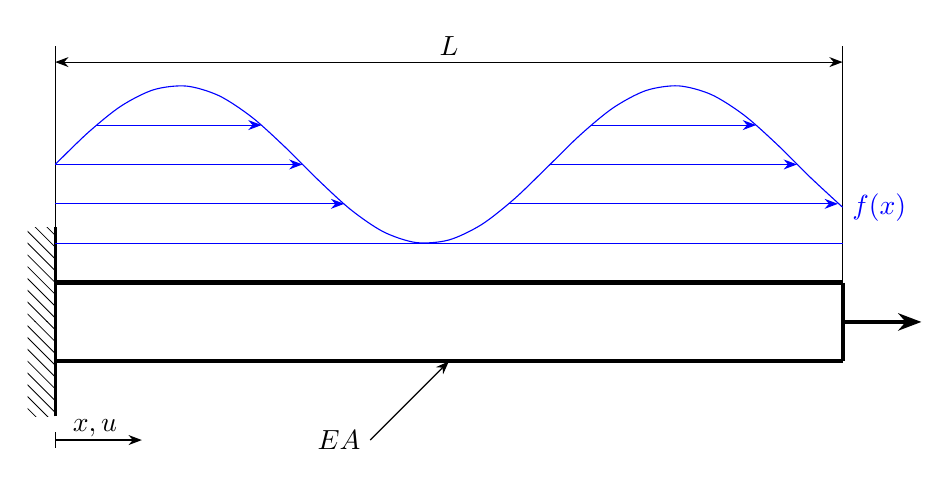
\begin{tikzpicture}[domain=0:10,smooth]
        %\draw[help lines,step =.5](-2 ,-2)grid(10 ,2);
        \point{a}{0}{0.6};
        \point{b}{0}{-0.6};
        \point{c}{0}{0.5};
        \point{d}{0}{-0.5};
        \point{e}{10}{0.5};
        \point{f}{10}{-0.5};
        \point{o}{0}{-1.5};
        \draw(0,-1.4)--(0,-1.6);
        \draw[-{Stealth}](0,-1.5)--(1.1,-1.5);
        \draw (0.1,-1.35) node[right] {$x,u$};
        %\node(0,0)node[left]{$x,u$};
        \support{3}{a}[270];
        \support{3}{b}[270];
        \beam{2}{c}{e};
        \beam{2}{e}{f};
        \beam{2}{f}{d};
        \draw(0,0)--(0,3.5);
        \draw(10,0)--(10,3.5);
        \draw [{Stealth}-{Stealth}](0,3.3)--(10,3.3);
        \draw (5,3.5) node[] {$L$};
        \draw[color=blue]   plot (\x,{sin(\x r)+2})    node[right] {$f(x)$};
        \draw[color=blue](0,1)--(10,1);
        \draw[color=blue,-{Stealth}](0,2)--(3.14,2);
        \draw[color=blue,-{Stealth}](6.28,2)--(9.42,2);
        \draw[color=blue,-{Stealth}](0,1.5)--(3.67,1.5);
        \draw[color=blue,-{Stealth}](5.76,1.5)--(9.94,1.5);
        \draw[color=blue,-{Stealth}](0.52,2.5)--(2.62,2.5);
        \draw[color=blue,-{Stealth}](6.81,2.5)--(8.9,2.5);
        \draw[very thick,-{Stealth}](10,0)--(11,0);
        \draw[{Stealth}-](5,-0.5)--(4,-1.5);
        \draw (4,-1.5) node[left] {$EA$};
    \end{tikzpicture}
    \caption{1D Truss}\label{fig:1dTruss}
\end{figure}

\noindent Strong form of the problem:


\begin{equation}\label{eq:StrongForm}
    \begin{aligned}
        -u''(x) &= f(x)  & \forall x\in [0,1] \\
        u(0)&=0\\
        u'(1)&=0\\
    \end{aligned}
\end{equation}

\noindent This equation can be used to model a 1D truss/bar with linear elastic properties.


\noindent If we suppose that $u$ is a solution for the strong form, given any function $v$, it is also true that:
\begin{equation*}
    -u''(x)v(x) = f(x)v(x) \quad \forall x\in [0,1]
\end{equation*}

\noindent If we integrate that expression in [0,1], we arrive at:
\begin{equation*}
    -\int_0^1 u''(x)v(x)dx = \int_0^1 f(x)v(x) dx
\end{equation*}

\noindent For that integrals to be well defined, we assume that $u\in H^2([0,1])$, $v\in H^1([0,1])$ and $f\in L^2([0,1])$. Then, we integrate by parts:
\begin{equation*}
    -[u'(x)v(x)]_{x=0}^{x=1}-\int_0^1 u'(x)v(x)'=dx \int_0^1 f(x)v(x) dx \quad\forall v\in H^1([0,1])
\end{equation*}
\begin{equation*}
    -u'(1)v(1)+u'(0)v(0)+\int_0^1 u'(x)v(x)'=dx \int_0^1 f(x)v(x) dx \quad\forall v\in H^1([0,1])
\end{equation*}

\noindent To force a solution that verifies the Dirichlet bound conditions, we define:
\begin{equation*}
    V=\{ v\in H^1([0,1]) \, : \, v(0)=0\}
\end{equation*}

\noindent Using that functional space and given that u'(1)=0, we then arrive at the weak form of the problem:
\begin{equation}
    \int_0^1 u'(x)v'(x)dx= \int_0^1 f(x)v(x) dx \quad\forall v\in V
\end{equation}

The model can be extended to take into consideration a diffusion coefficient $\beta$, a mass coefficient $\alpha$, and an inhomogeneous density $c(x)$.

\begin{equation}
    \frac{d}{dx}\bigg( c(x) \frac{d u(x)}{dx} \bigg) + \alpha \frac{d u(x)}{dx} + \beta u(x) = f(x)
\end{equation}
The derivation of the weak form is analogous to the previous one, leading to the following result:

\begin{equation}
    \big(-K + \alpha D + \beta M\big) \mathbf{u} = \mathbf{F}
\end{equation}

where $K$, $D$, and $M$ are the stiffness matrix, the diffusion matrix, and the mass matrix, respectively. 

\begin{align*}
    K_{ij} &= \int_{\Omega} \frac{d \phi_i}{dx} \frac{d \phi_j}{dx} c(x) \, dx \\
    D_{ij} &= \int_{\Omega} \frac{d \phi_i}{dx} \phi_j \, dx \\
    M_{ij} &= \int_{\Omega} \phi_i \phi_j \, dx 
\end{align*}

The force vector has the same expression as before:

\begin{equation}
    F_i = \int_{\Omega} f(x) \phi_i \, dx
\end{equation}


\section{FEM with first order Lagrange elements}
\noindent Solve:
\begin{equation*}
    \textbf{A}x=b
\end{equation*}

\noindent Where:
\begin{equation*}
    \textbf{A}=[a_{ij}]
\end{equation*}

\begin{equation}
\begin{gathered}
     a_{ij}=\int_a^b \varphi_j' \varphi_i' dx \;\;\;\;\text{if } j\in\{ i-1,i,i+1\}  \\
     a_{ij}=0 \;\;\;\;\text{if } j\notin\{ i-1,i,i+1\} \\
     b=[b_i], \quad b_{i}=\int_a^b f \varphi_i dx \quad
     i=1,...,N+1 \\
     b_1 = b_{N+1} = 0 
\end{gathered}
\end{equation}



\noindent The functions $\varphi_i$ are defined as:
\[\varphi_i= \left\{
\begin{array}{rcl}
\frac{x-x_{i-1}}{x_{i+1}-x_{i}}& \text{if } x\in [x_{i-1}, x_i]\\
\frac{x_{i+1}-x}{x_{i+1}-x_{i}}& \text{if } x\in [x_{i}, x_{i+1}]\\
0& \text{if } x\notin [x_{i-1}, x_{i+1}]
\end{array}\right.\]

\noindent The previous linear system can be assembled with the help of an element stiffness matrix [2x2] and an element force vector [2x1]. For the element $i$, which nodes are $[x_i,x_{i+1}]$, the element stiffness matrix and force vector are defined as follows.

\begin{equation*}
    {K}^e=[K^i_{lk}]=\int_{x_i}^{x_{i+1}} \varphi_{i-1+l}' \varphi_{i-1+k}' dx \quad
     l,k=1,2  
\end{equation*}

\begin{equation*}
    b^e=[b^i_{l}]=\int_{x_i}^{x_{i+1}} \varphi_{i-1+l} f dx \quad
     l=1,2  
\end{equation*}

\noindent The assembly of the stiffness matrix in global coordinates is:
\begin{gather*}
    K=\begin{pmatrix}
        K_{11}^1 & K_{12}^1 & 0 & 0 & \cdots & 0\\
        K_{21}^1 & K_{22}^1+K_{11}^2 & K_{12}^2 & 0 & \cdots & 0\\ 
        0 & K_{21}^2 & K_{22}^2+K_{11}^3 & K_{12}^3 & \cdots & 0\\
        \vdots & \vdots & \vdots & \vdots & \ddots & \vdots\\
        0 & 0 & 0 & 0 & \cdots & K_{22}^N
    \end{pmatrix}
\end{gather*}

\noindent And the assembly of $b$ terms has the structure:
\begin{gather*}
    b=\begin{pmatrix}
        b_1^1\\b_2^1+b_1^2\\b_2^2+b_1^3\\ \vdots \\ b_2^N
    \end{pmatrix}
\end{gather*}

\noindent As there is no mass matrix in this problem nor bound conditions to be added, we take $A=K$. And so, the FEM problem to solve is:
\begin{gather*}
    Ac=b
\end{gather*}

\noindent Which leads to the solution:
\begin{equation*}
    u^h=\sum\limits_{i=1}^{N+1} c_i\psi_i(x)
\end{equation*}
\end{document}
